\documentclass[aspectratio=169]{beamer}
\setbeamertemplate{navigation symbols}{}
\usepackage{color, amsmath, comment, subfigure}
\usepackage{url}

\usepackage{hyperref}
\hypersetup{
    colorlinks=true,
    linkcolor=blue,
    filecolor=magenta,      
    urlcolor=cyan,
}

%%%%%%%%%%%%%%%%%%%%%%%%%%
\title[]{Class slides for Tuesday, September 22:\\Armed conflict, part 1}
\author[]{Matthew J. Salganik}
\institute[]{}
\date[]{COS 597E/SOC 555 Limits to prediction\\Fall 2020, Princeton University}

\begin{document}
%%%%%%%%%%%%%%%%%%%%%%%%%%%
\frame{\titlepage}
%%%%%%%%%%%%%%%%%%%%%%%%%%%
\begin{frame}
\frametitle{}

\begin{center}
\only<1>{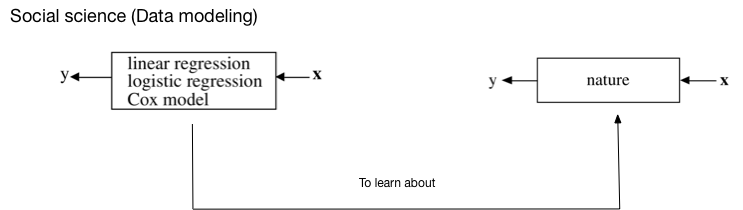
\includegraphics[width=0.9\textwidth]{figures/third_way_1}}%
\only<2>{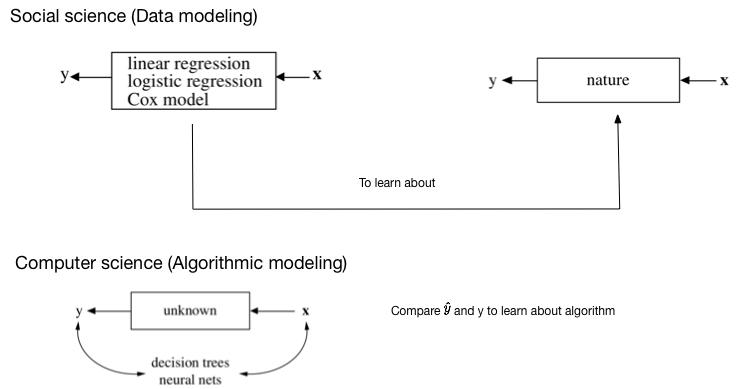
\includegraphics[width=0.9\textwidth]{figures/third_way_2}}%
\only<3>{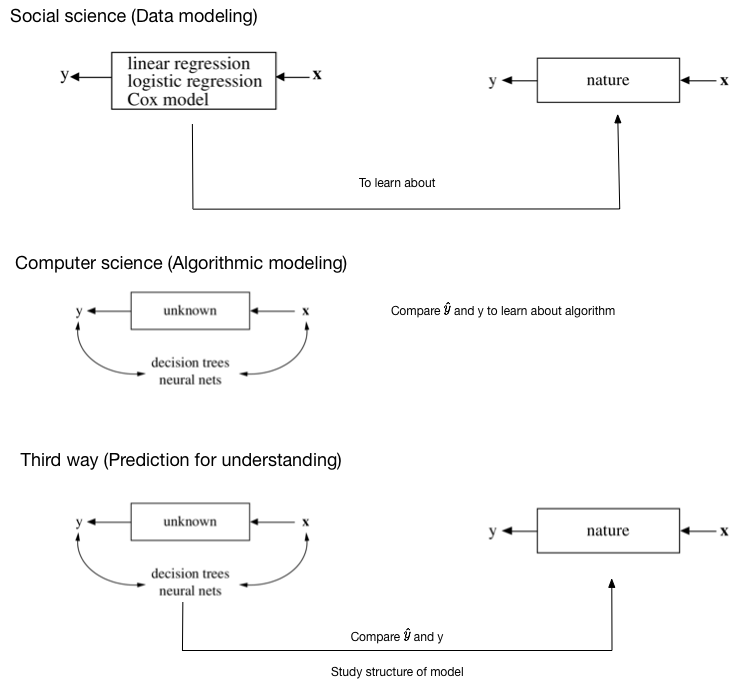
\includegraphics[width=0.6\textwidth]{figures/third_way_3}}%
\end{center}

\end{frame}
%%%%%%%%%%%%%%%%%%%%%%%%%%%
\begin{frame}
\frametitle{}

\begin{center}
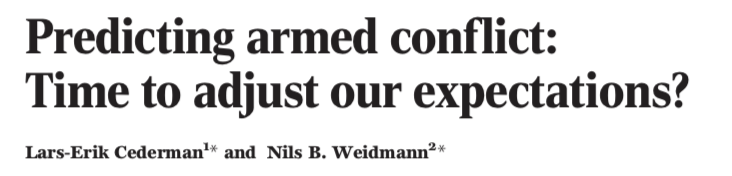
\includegraphics[width=0.9\textwidth]{figures/cederman_predicting_2017_title}
\end{center}

\end{frame}
%%%%%%%%%%%%%%%%%%%%%%%%%%%
\begin{frame}
\frametitle{}

\begin{itemize}
\item Prediction can be at different timescales (daily, weekly, yearly) or different geographic scales (cities, states, countries).  Some geographic and timescales may be more accurate than others.  Some types of violence may also be more predictable than others (e.g., violence between nation-states vs violence by ``terrorist'' groups)
\pause
% Nice place to talk about lumpers and splitters
\item Prediction of armed conflict will be difficult because: 
\begin{itemize}
\item complexity of the data generating process (this is asserted but not explained)
\item historical disjunctures (e.g., end of Soviet Union, countries merging and splitting) 
\item data quality (both outcomes and predictors)
\item rare events
\end{itemize}
\pause
\item As a thought experiment compare predicting armed conflict to predicting US Presidential election.
\pause
\item Even if we had a perfectly accurate predictions, this might not be very useful for policy or theory.
\end{itemize}

\end{frame}
%%%%%%%%%%%%%%%%%%%%%%%%%%%
\begin{frame}

\begin{center}
Impossibility result in Gartzke \& Coletta and Gartzke
\end{center}

\end{frame}
%%%%%%%%%%%%%%%%%%%%%%%%%%%
\begin{frame}

\begin{itemize}
\item These kinds of limits to prediction arguments are very rare in the social sciences.
\pause
\item $U_A(d) = Pr(\text{war})[\text{expected value from war}] + [1 - Pr(\text{war})][\text{value from accepted demand}]$
\pause
\item Demand from actor A depends on the unseen (and unobservable) costs of for actor $B$.
\pause
\item Sketch: If motivated participants can't do it, then researchers can't do it. 
\pause
\item Limitations:
  \begin{itemize}
  \item hard to put a number on the unpredictability
  \pause
  \item beware of tweaks to the set-up (e.g, repeated games, changes to the utility function)
  \pause
  \item What about divorce? \pause What about chess?
\end{itemize}
\end{itemize}

\end{frame}
%%%%%%%%%%%%%%%%%%%%%%%%%%%
\begin{frame}

\begin{center}
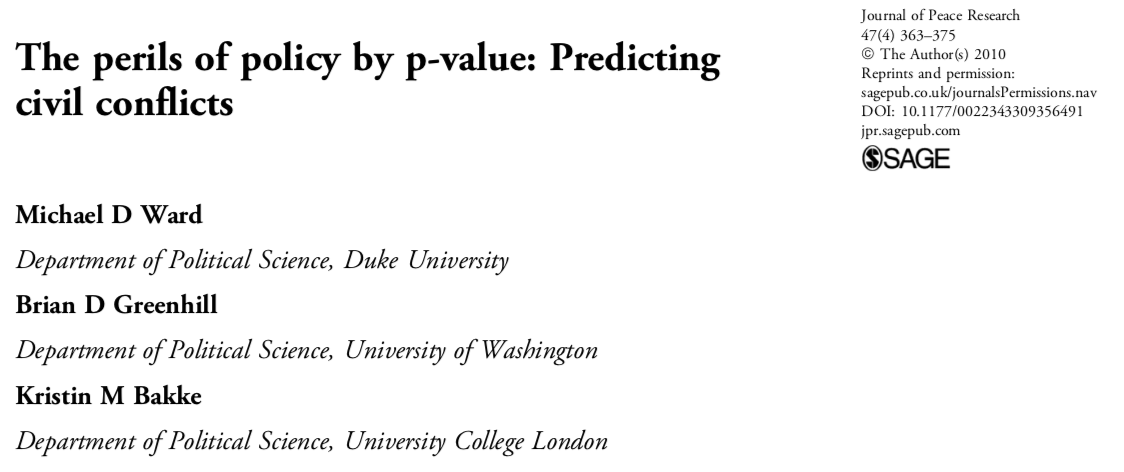
\includegraphics[height=0.7\textheight]{figures/ward_perils_2010_title}
\end{center}

\end{frame}
%%%%%%%%%%%%%%%%%%%%%%%%%%%
\begin{frame}

\begin{itemize}
\item Bring $\hat{y}$ into $\hat{\beta}$ world
\pause
\item social scientists often says that a variable X predicts Y if X is statistically significant in a regression model to prediction Y.
\pause
\item assess model not by whether it produces new predictors that are statistically significant, but by whether it adds to predictive power.
\pause
\item They don't call for turning civil war prediction into a Kaggle contest.
\end{itemize}

\end{frame}
%%%%%%%%%%%%%%%%%%%%%%%%%%%
\begin{frame}

Provocations:
\begin{itemize}
\item Maybe we can isolate unpredictability? peace $\rightarrow$ crisis $\rightarrow$ war.  Gartzke argues we can predict peace $\rightarrow$ crisis, but not crisis $\rightarrow$ war.  Maybe we could test that empirically?
\pause
\item How can we limit ourselves to ``useful'' improvements in predictive performance?
\pause
\item Can a model (e.g., Fearon \& Laitin and Collier \& Hoefller) aid ``understanding'' even if it does not predict accurately?
\pause
\item What should we do when we can't just get more cases?
\end{itemize}

\end{frame}
%%%%%%%%%%%%%%%%%%%%%%%%%%%


\frame{\titlepage}


\end{document}
